\documentclass[11pt]{article}
\usepackage{mystyle}

\title{Towards whole-brain validation of diffusion MRI fiber orientation
  distributions with x-ray microcomputed tomography}
\author{Scott Trinkle, Sean
  Foxley, Narayanan Kasthuri and Patrick La Riv\`iere}
\date{Last edited: \today}

\begin{document}

\maketitle

\textbf{Note:} This document is a loosely-organized collection of everything I
have written regarding the validation of HARDI ODFs/FODs with microCT data using
structure tensor analysis. Some of it borrows heavily/directly from other
papers, most notably Schilling et al. 2018 \cite{Schilling2018} (validating
HARDI with 3D histology) and Alimi et al. 2018 \cite{Alimi2018} (all of
spherical harmonic discussion in section \ref{alimi}).


\section{Introduction}
Diffusion MRI (dMRI) is a powerful, non-invasive tool for characterizing
three-dimensional (3D) tissue microstructure on a macroscopic scale, and is
widely used in both research and clinical settings. New methods of
reconstructing 3D fiber orientation distributions (FODs) from dMRI data are
rapidly being developed, each based on the assumption that the diffusion
contrast from dMRI provides an accurate representation of the underlying
anatomical fiber structure. Previous efforts to validate these FODs have relied
on ground truth histological data with non-isotropic resolution over small
regions of interest (ROI). In this study, we demonstrate a pipeline for the use
of natively isotropic, synchrotron-based x-ray microcomputed tomography data to
validate FODs over a whole mouse brain.

\section{Methods}
\subsection{MRI}
\subsubsection{Acquisition}
A post-mortem brain was scanned on a Bruker 9.4 T magnet with a 3D
diffusion-weighted spin-echo sequence at 150 $\upmu$m isotropic
resolution. Data was acquired at a b-value of 3000 s/mm$^2$ over 30 uniformly
distributed directions.

\subsubsection{MRI reconstruction methods}
The MRI ODFs were reconstructed from the dMRI data using diffusion tensor
imaging (DTI) \cite{Basser1994}, constrained spherical deconvolution (CSD)
\cite{Tournier2004}, Q-ball imaging, constant solid angle (CSA)
\cite{Aganj2010}, and the sparse fascicle model (SFM) \cite{Rokem2015}. All
reconstructions were performed using the open-source Dipy Python package
\cite{Garyfallidis2014}.

\subsection{X-ray}
\subsubsection{Acquisition}
The specimen was then stained with uranyl acetate,
osmium tetroxide and lead citrate in preparation for x-ray imaging at the
Advanced Photon Source at Argonne National Lab. The x-ray data was acquired
using a mosaic stitching method, yielding an image volume over the whole brain
with 1.2 $\upmu$m isotropic resolution.


\subsection{Structure Tensor Analysis}
Structure tensor analysis was initially developed in a 1987 computer vision
paper by Bigun and Granlund~\cite{Bigun1987}. It has since been used for a
variety of computer vision and materials science applications, including finding
the orientation of textile fibers with synchrotron microCT
imaging~\cite{Straumit2015}. It was notably applied to validating diffusion MRI
with 2D histology by Budde~\cite{Budde2012,Budde2013} and
others. Schilling~\cite{Schilling2016,Schilling2018} and Khan~\cite{Khan2015}
have extended the analysis to 3D for the same purpose.

\subsubsection{Derivation}

Consider a three-dimensional intensity image, $f(x,y,z)$, with gradient:
\begin{align}
  \label{eq:grad}
  \nabla f_{\sigma_d} = {\left(f_x, f_y, f_z\right)}^T
\end{align}
which is calculated using Gaussian derivative filters:
\begin{align}
  \label{eq:gradcomps}
  f_x = g_{x,\sigma_d} \ast f & &  f_y = g_{y,\sigma_d} \ast f & &  f_z = g_{z,\sigma_d} \ast f
\end{align}
where $\ast$ denotes the convolution operator and $g_{i, \sigma_d}$ denotes the
spatial derivative in the $i$-direction of a 3D~Gaussian with
standard deviation $\sigma_d$:
\begin{align}
  \label{eq:gauss}
  g_{i,\sigma_d} &= \frac{\partial}{\partial i}\left(\frac{1}{\left(2\pi\sigma_d^2\right)^{3/2}}\text{ exp}\left\{-\frac{x^2 + y^2 + z^2}{2\sigma_d^2}\right\}\right), & i \in [x, y, z]
\end{align}

The image gradient is used to construct a ``gradient square tensor'' by taking
the dyadic product of the gradient vector with itself:
\begin{align}
  \label{eq:GST}
  \text{GST}_{\sigma_d} = \nabla f_{\sigma_d} \nabla f_{\sigma_d}^T =
  \begin{pmatrix}
    f_x^2 & f_x f_y & f_x f_z \\
    f_x f_y & f_y^2 & f_y f_z \\
    f_x f_z & f_y f_z & f_z^2 \\
  \end{pmatrix}
\end{align}

Each element of the GST is then averaged over a local neighborhood to create the
voxel-wise structure tensor. This averaging is typically performed using a 3D
Gaussian filter with standard deviation $\sigma_N$:
\begin{align}
  \label{eq:ST}
  \text{ST}_{\sigma_N}\left(\nabla f_{\sigma_d}\right) = g_{\sigma_N} \ast
  \left(\nabla f_{\sigma_d} \nabla f_{\sigma_d}^T \right) = g_{\sigma_N} \ast
  \begin{pmatrix}
    f_x^2 & f_x f_y & f_x f_z \\
    f_x f_y & f_y^2 & f_y f_z \\
    f_x f_z & f_y f_z & f_z^2 \\
  \end{pmatrix}
\end{align}

This results in a 3$\times$3 symmetric, positive semi-definite, rank-two tensor
at every voxel. The direction of minimal intensity variation is given by the
eigenvector of this tensor corresponding to the smallest eigenvalue. We make the
assumption that this direction also describes the corresponding fiber
orientation of that voxel.

The eigenvalues can be used to estimate the certainty in the estimated fiber
orientation with a voxel-wise anisotropy measure. Here, we use fractional
anisotropy (FA), a metric that is also used in MRI diffusion tensor imaging (DTI):
\begin{align}
  \label{eq:FA}
  \text{FA} = \sqrt{\frac{1}{2}\frac{(\lambda_1-\lambda_2)^2 + (\lambda_2-\lambda_3)^2 +
      (\lambda_1 - \lambda_3)^2}{\lambda_1^2 + \lambda_2^2 + \lambda_3^2}}
\end{align}
where $\lambda_1$, $\lambda_2$ and $\lambda_3$ are the primary, secondary and
tertiary eigenvalues of the structure tensor.

The FA is commonly used to threshold the image $f$, so voxels with low
anisotropy are not included in the orientation distribution.

\subsubsection{Construction of X-ray ODF}\label{alimi}
The structure tensor analysis generates a principal orientation
vector at each voxel. Alimi et al. \cite{Alimi2018} describe how
an ODF can be generated over a 3D ROI by binning the vectors from the X-ray data
into a spherical histogram expanded on the real spherical harmonics (SH).


The spherical harmonics are defined as
\begin{align}
  Y_l^m(\theta, \phi) = N_l^m P_l^m(\text{cos}\theta)e^{jm\phi},
\end{align}
where $N_l^m$ is a normalization coefficient, $P_l^m$ are the
associated Legendre polynomials, and $\theta \in [0, \pi]$ and $\phi \in [0, 2\pi]$
are the polar and azimuth angles, respectively. 
The SH form an orthonormal basis over $L_2(\mathbb{S}^2)$. Any
square integrable function $g(\theta, \phi) \in L_2(\mathbb{S}^2)$ can
be expressed as a linear combination of SH:
\begin{align}
  g(\theta, \phi) = \sum_{l=0}^{\infty}\sum_{m=-l}^l c_{lm}Y_l^m(\theta, \phi),
  \label{eq:SHexpand}
\end{align}
with coefficients $c_{lm}$ given by
\begin{align}
  c_{lm} = \int_{\mathbb{S}^2} g(\bm{w}) \bar{Y}_l^m(\bm{w}) \mathrm{d}\bm{w},
  \label{eq:coeffs_0}
\end{align}
where the overbar denotes conjugation and
\begin{align}
  \bm{w}(\theta, \phi) = [\text{sin}\theta\text{cos}\phi\text{, }  \text{sin}\theta \text{sin}\phi\text{, }  \text{cos}\theta]^T.
\end{align}

We can model each orientation vector in an X-ray ROI as a Dirac delta function
$\delta$ on the sphere. That is, in a ROI containing $K$ voxels, our ODF
can be written as
\begin{align}
  \text{ODF}(\theta, \phi) = \frac{1}{K}\sum_{k=1}^K \delta(\theta - \theta_k)\delta(\phi - \phi_k).
\end{align}

If we substitute this into Eqn \ref{eq:coeffs_0}, then the sifting property of the Dirac
delta function can be used, and the integral reduces to:
\begin{align}
  c_{lm} = \frac{1}{K}\sum_{k=1}^K \bar{Y}_l^m(\theta_k, \phi_k).
  \label{eq:get_coeffs}
\end{align}
A SH approximation $\hat{\text{ODF}}(\theta, \phi)$ can then be determined to an arbitrary
band-limit $L_{max}$ using Eqn \ref{eq:SHexpand}.

Spherical harmonics are used extensively in the HARDI literature
to represents ODFs \cite{Tournier2004}. Generally, it is assumed that diffusion is symmetric
about the origin, so odd-ordered SH components are assumed to be zero and ignored. Furthermore,
since the diffusion-weighted signal and ODF are both real functions, their SH representations
exhibit conjugate symmetry:
\begin{align}
  Y_{l}^m(\theta, \phi)_{real} \equiv
  \begin{cases}
    \sqrt{2}\text{Re}\left[Y_l^{|m|}(\theta, \phi)\right] & m < 0\\
    Y_l^0(\theta, \phi) & m = 0\\
    \sqrt{2}\text{Im}\left[Y_l^m(\theta, \phi)\right] & m > 0\\
  \end{cases}
  \label{eq:real_Y}
\end{align}

These simplifications hold true for the X-ray ODFs as well. In this work, we use a
band-limit of $L_{max} = 20$, for a total number of 231 even-ordered SH coefficients. 

\subsection{Comparison Metrics}
A number of features were calculated from the MRI and X-Ray ODFs. A peak finding
algorithm implemented in the Dipy python package \cite{Garyfallidis2014} was
used to identify the orientations of distinct fiber populations. In this
algorithm, peaks are defined as points on the ODF that are greater than at least
one neighbor and greater than or equal to all neighbors. Peaks are discarded if
they are below a threshold percentage of 20\% of the maximum peak value and
within a minimum separation angle of 20$^{\circ}$. These threshold values are
commonly seen in the literature \cite{Daducci2014, Schilling2018}.

To evaluate agreement in overall shape between ODFs, the angular correlation coefficient
(ACC) and Jensen-Shannon divergence (JSD) are implemented. The ACC is analogous to
a linear correlation coefficient and can be calculated directly from the SH
coefficients of the two ODFs \cite{Anderson2005}. Given SH coefficients $u_{lm}$ and $v_{lm}$ for
two respective ODFs, the ACC is calculated as:
\begin{align}
  \text{ACC} = \frac{\sum\limits_{l=1}^{L_{max}}\sum\limits_{m=-l}^l u_{lm}\bar{v}_{lm}}{\left[\sum\limits_{l'=1}^{L_{max}}\sum\limits_{m'=-l'}^{l'}|u_{l'm'}|^2\right]^{1/2}\left[\sum\limits_{l'=1}^{L_{max}}\sum\limits_{m'=-l'}^{l'}|\bar{v}_{l'm'}|^2\right]^{1/2}}.
\end{align}
The JSD measures the distance between two probability distributions and has also
been widely used in the dMRI literature \cite{Cohen-Adad2011}. The ODFs are projected onto
$N$ values equally distributed over a sphere using a Fibonacci sampling algorithm [CITE?].
The JSD is then defined as
\begin{align}
  \text{JSD}(P, Q) = \frac{D_{KL}(P, M) + D_{KL}(Q, M)}{2},
\end{align}
where
\begin{align}
  M_i = \frac{P_i + Q_i}{2},
\end{align}
$P_i$ and $Q_i$ are the magnitudes of the X-ray and MRI ODFs along index
$i \in [1, N]$, and $D_{KL}$ is the Kullback-Leibler divergence [CITE?]:
\begin{align}
  D_{KL}(P, Q) = \sum_i P_i\text{log}\left(\frac{P_i}{Q_i}\right).
\end{align}
The JSD is bounded between 0 and 1, where lower values indicate greater
similarity of distributions.

\section{Sensitivity Study}
A number of tests were performed to understand the sensitivity of the final
X-ray ODFs and identified peaks to the various parameters in the structure
tensor analysis pipeline: specifically the choice of the smoothing factors
$\sigma_D$ and $\sigma_N$. 

\subsection{Phantom creation}

First, several digital phantoms were created to investigate the effects of
different fiber conditions. A sample ROI roughly the size of a single MRI voxel
was taken from the X-ray data. K-means segmentation was performed to segment the
vasculature and nerve fibers. A sample slice with both vasculature and fiber
masks is shown in Figure \ref{fig:xrayslice}.

\begin{figure}[h]
  \centering
  \begin{subfigure}[b]{0.3\textwidth}
    \centering
    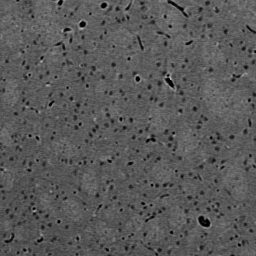
\includegraphics[width=0.9\linewidth]{figs/xray_sl84}
    \caption{X-ray ROI slice.}
    \label{fig:xraydata}
  \end{subfigure}
  \hspace{1em}
  \begin{subfigure}[b]{0.3\textwidth}
    \centering
    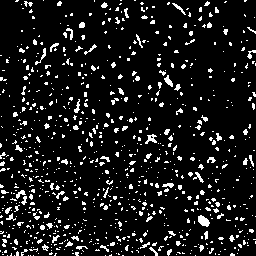
\includegraphics[width=0.9\linewidth]{figs/vasc_mask84}
    \caption{Segmented vasculature mask.}
    \label{fig:vascmasc}
  \end{subfigure}
  \hspace{1em}
  \begin{subfigure}[b]{0.3\textwidth}
    \centering
    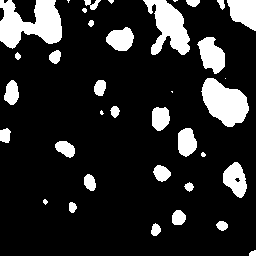
\includegraphics[width=0.9\linewidth]{figs/fibmask84}
    \caption{Segmented fiber mask.}
    \label{fig:fibmask}
  \end{subfigure}
  \caption{Sample X-ray slice with vasculature and fiber masks.}
  \label{fig:xrayslice}
\end{figure}

The simulated $150\times150\times150$ $\upmu$m$^3$ (the size of one MRI voxel)
phantoms were then constructed using a random Poisson-distributed background
with the same mean as the background in the real data, overlaid with random
Poisson distributed values within the raw vasculature mask using the real data
vasculature mean, and custom-defined cylindrical nerve fibers, also using random
Poisson-distributed values with the same mean as the real data.

Four phantoms were constructed that included nine parallel fibers along the
x-axis (left to right in Figure \ref{fig:xraydata}) with radii of 4.8, 9.6, 14.4
and 19.2 $\upmu$m, and eight phantoms were constructed that simulated four
parallel fibers along the z-axis (in and out of the page in Figure
\ref{fig:xraydata}) and four parallel fibers at a specified angle off the
z-axis, from 25$^{\circ}$ to 85$^{\circ}$, every 10$^{\circ}$. All fibers in the
crossing angle phantoms had a radius of 9.6 $\upmu$m. Sample slices from a
45$^{\circ}$ crossing fiber phantom and a single fiber population phantom (r =
9.6 $\upmu$m) are shown in Figure \ref{fig:phantoms}.

\begin{figure}[H]
  \centering
  \begin{subfigure}[t]{0.35\textwidth}
    \centering
    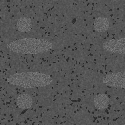
\includegraphics[width=0.9\linewidth]{figs/deg45}
    \caption{45$^{\circ}$ phantom.}
    \label{fig:deg45}
  \end{subfigure}
  \hspace{1em}
  \begin{subfigure}[t]{0.35\textwidth}
    \centering
    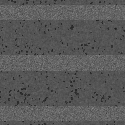
\includegraphics[width=0.9\linewidth]{figs/r8}
    \caption{Single fiber population phantom, r = 9.6 $\upmu$m.}
    \label{fig:r8}
  \end{subfigure}
  \caption{Sample crossing fiber and single fiber population phantoms.}
  \label{fig:phantoms}
\end{figure}

\subsection{True phantom ODFs}

With the orientations of the phantom fiber populations known exactly, the true
ODFs could be calculated and compared with those calculated using structure
tensor analysis. For each phantom, the number of voxels in the various fiber
population masks was used along with the true orientations of those fiber
populations to create a vector of true~($\theta$, $\phi$) values. These values
were then expanded on SH up to $L_{max}=20$ as in Equation~\ref{eq:get_coeffs}.
The true ODFs for the phantoms shown in Figure~\ref{fig:phantoms} are shown in
Figure~\ref{fig:true_odfs}. 

\begin{figure}[h]
  \centering
  \begin{subfigure}[t]{0.35\textwidth}
    \centering
    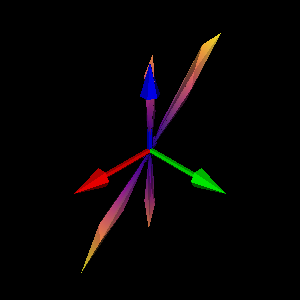
\includegraphics[width=0.9\linewidth]{figs/deg45_ODF}
    \caption{True ODF for 45$^{\circ}$ phantom.}
    \label{fig:deg45odf}
  \end{subfigure}
  \hspace{1em}
  \begin{subfigure}[t]{0.35\textwidth}
    \centering
    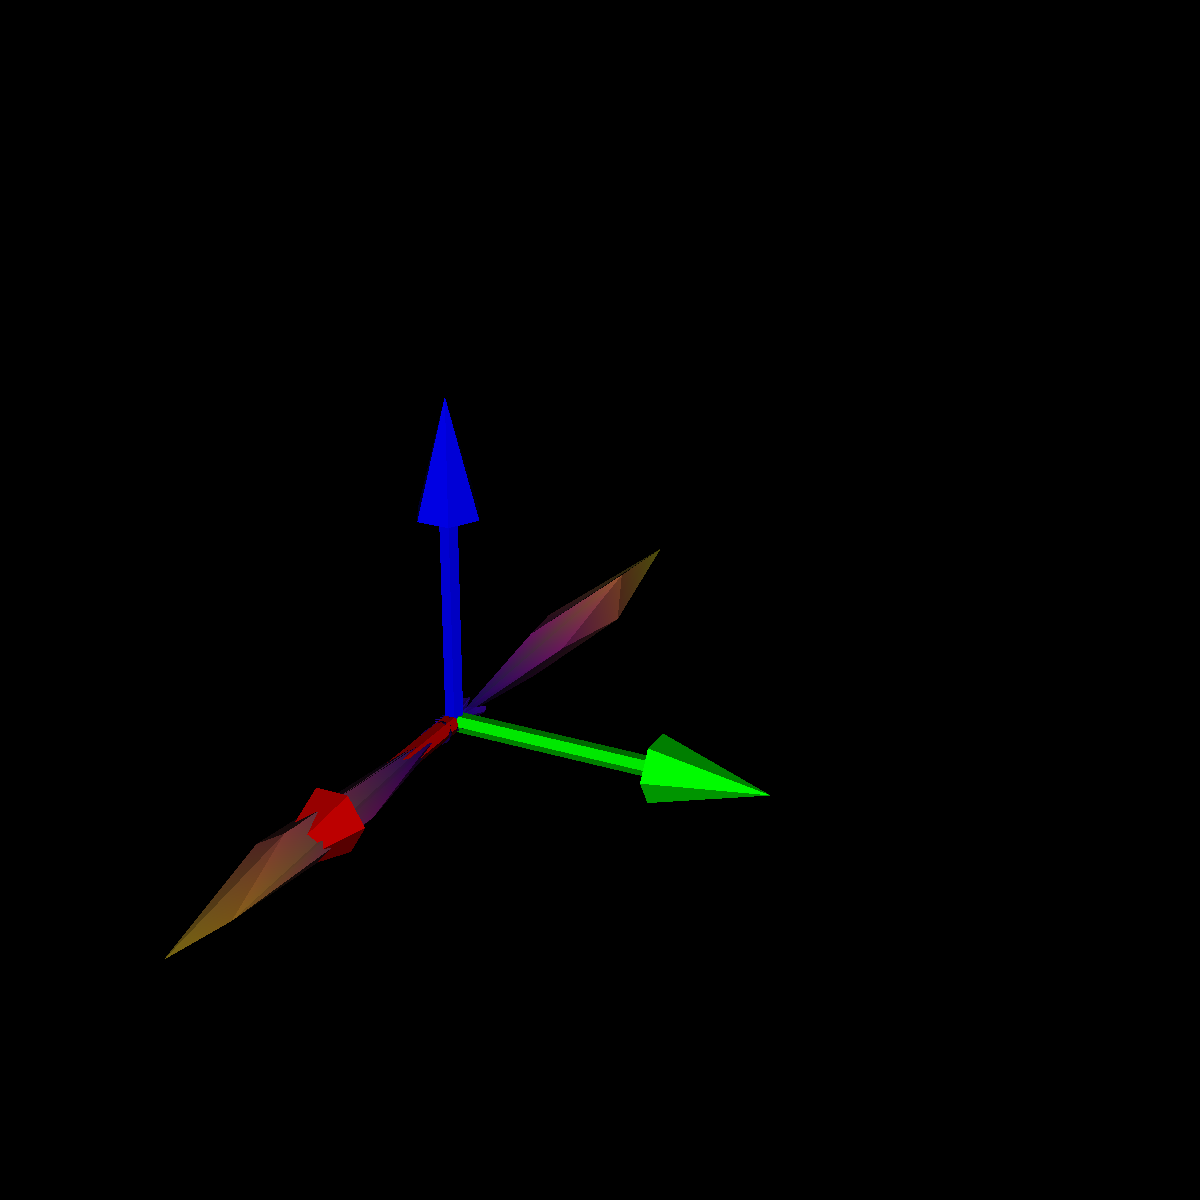
\includegraphics[width=0.9\linewidth]{figs/r8_ODF}
    \caption{True ODF for single fiber population phantom, r = 8 pixels.}
    \label{fig:r8odf}
  \end{subfigure}
  \captionsetup{width=0.7\textwidth}
  \caption{Sample true ODFs for crossing fiber and single fiber population
    phantoms.  SH components were calculated up to $L_{max}=20$ and represented
    here on a sphere with $N$=1500 points.}
  \label{fig:true_odfs}
\end{figure}

\subsection{Comparison with structure tensor ODFs}
The ODF was then calculated for each phantom using structure tensor analysis,
with values of $\sigma_D$ from 1--10~$\upmu$m spaced 0.5~$\upmu$m apart,
and values of $\sigma_N$ from 2--12~$\upmu$m spaced 0.5~$\upmu$m apart, for a total
of~399 combinations per phantom.

A number of evaluation metrics were calculated for each combination of $\sigma$
values.  The total number of identified peaks was calculated, as well as the
angular error between the peak locations calculated from the structure tensor
and true ODFs (for the crossing fiber phantoms, the angular error was averaged
between the two peaks).  The ACC and JSD were used to compare the overall shape
of the ODFs. For a good choice of $\sigma$ values, the voxels within a nerve
fiber should have a higher FA value than voxels in the background. To assess
this, ROC analysis was performed to evaluate the ability to classify nerve
fibers in each phantom by the FA value. The area under the ROC curve (AUC) was
then used as an evaluation metric.

Color plots and summary scatter plots of each metric and phantom are shown in
Figures~\ref{fig:angle_results}-\ref{fig:angle_max_inds}
and~\ref{fig:size_results}-\ref{fig:size_max_inds} for crossing fiber and single
fiber phantoms, respectively.

For each color plot, $\sigma_D$ is on the x-axis and $\sigma_N$ is on the
y-axis. Rows from top to bottom indicate either increasing crossing angle or
increasing fiber radius. High values are desired for ACC and AUC, while low
values are desired for JSD and Peak Error. For ease in visualization, the
colormaps for JSD and Peak Error are inverted such that bright/yellow colors
indicate good performance across all metrics. Grey pixels indicate combinations
of $\sigma_D$ and $\sigma_N$ that led to an incorrect identification of the
number of peaks in the ODF. The number and location of peaks are key metrics
that will eventually be used in comparing X-ray ODFs to MRI ODFs, so these
values are excluded.

For the scatter plots, the $\sigma_D$, $\sigma_N$ combination corresponding to the
maximum (or minimum, for JSD and Peak Error) metric value are plotted for each
metric and each phantom. The color of each point corresponds to either crossing
angle or fiber radius, and the shape corresponds to the evaluation metric. Note that
some of these metrics do not have a well-defined peak, so the ``optimal'' choice
is somewhat arbitrary. 

\newpage
\begin{center}
  \captionsetup{width=0.9\textwidth} \captionof{figure}{Parameter evaluation
    metrics for crossing fiber phantoms. Rows indicate crossing angle between
    fiber populations. Columns indicate evaluation metrics. Colormaps are
    inverted for metrics that are desired to be low (JSD and Peak Error)}
  \begin{longtable}{cccc}
    AUC & Peak Error & ACC & JSD\\
    \im{0.24}{\anglepath{15}{AUC}} & \im{0.24}{\anglepath{15}{ODF_Peak_Error}} & \im{0.24}{\anglepath{15}{ACC}} & \im{0.24}{\anglepath{15}{JSD}}\\
    \im{0.24}{\anglepath{25}{AUC}} & \im{0.24}{\anglepath{25}{ODF_Peak_Error}} & \im{0.24}{\anglepath{25}{ACC}} & \im{0.24}{\anglepath{25}{JSD}}\\
    \im{0.24}{\anglepath{35}{AUC}} & \im{0.24}{\anglepath{35}{ODF_Peak_Error}} & \im{0.24}{\anglepath{35}{ACC}} & \im{0.24}{\anglepath{35}{JSD}}\\
    \im{0.24}{\anglepath{45}{AUC}} & \im{0.24}{\anglepath{45}{ODF_Peak_Error}} & \im{0.24}{\anglepath{45}{ACC}} & \im{0.24}{\anglepath{45}{JSD}}\\
    \im{0.24}{\anglepath{55}{AUC}} & \im{0.24}{\anglepath{55}{ODF_Peak_Error}} & \im{0.24}{\anglepath{55}{ACC}} & \im{0.24}{\anglepath{55}{JSD}}\\
    \im{0.24}{\anglepath{65}{AUC}} & \im{0.24}{\anglepath{65}{ODF_Peak_Error}} & \im{0.24}{\anglepath{65}{ACC}} & \im{0.24}{\anglepath{65}{JSD}}\\
    \im{0.24}{\anglepath{75}{AUC}} & \im{0.24}{\anglepath{75}{ODF_Peak_Error}} & \im{0.24}{\anglepath{75}{ACC}} & \im{0.24}{\anglepath{75}{JSD}}\\
    \im{0.24}{\anglepath{85}{AUC}} & \im{0.24}{\anglepath{85}{ODF_Peak_Error}} & \im{0.24}{\anglepath{85}{ACC}} & \im{0.24}{\anglepath{85}{JSD}}
  \end{longtable}
  \label{fig:angle_results}
\end{center}

\begin{figure}[h]
  \centering
  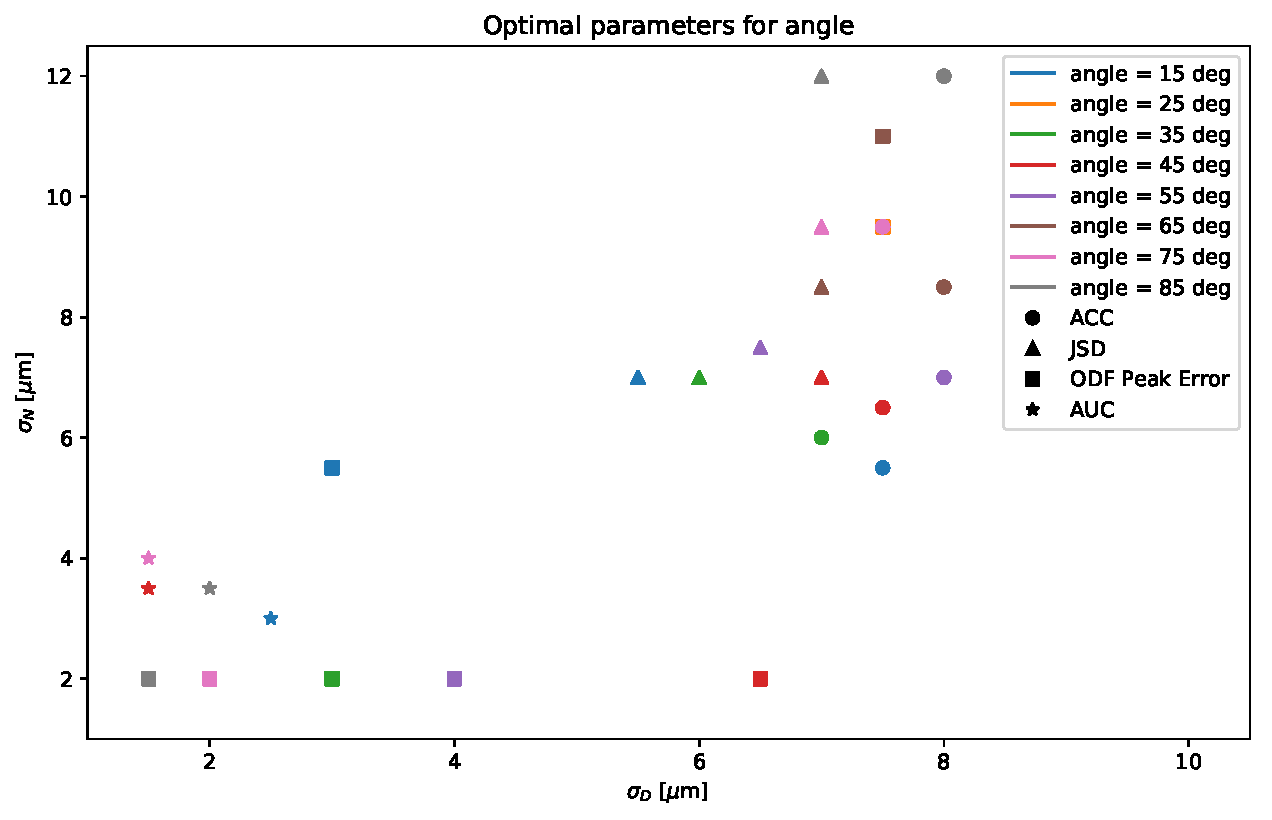
\includegraphics[width=0.70\linewidth]{../analysis/by_angle_results/angle_best_params}
  \captionsetup{width=0.7\linewidth}
  \caption{Summary of Figure~\ref{fig:angle_results}. Each point indicates the
    $\sigma_D$, $\sigma_N$ pair that maximizes a given metric for a given
    phantom. Different colors indicate different crossing angles and different
    shapes indicate different metrics.}
  \label{fig:angle_max_inds}
\end{figure}

\begin{center}
  \captionsetup{width=0.90\textwidth} \captionof{figure}{Parameter evaluation
    metrics for single fiber population phantoms. Rows indicate fiber
    radius. Columns indicate evaluation metrics. Colormaps are inverted for
    metrics that are desired to be low (JSD and Peak Error)}
  \begin{longtable}{cccc}
    AUC & Peak Error & ACC & AUC\\
    \im{0.24}{\sizepath{4_8}{AUC}} & \im{0.24}{\sizepath{4_8}{ODF_Peak_Error}} & \im{0.24}{\sizepath{4_8}{ACC}} & \im{0.24}{\sizepath{4_8}{JSD}}\\
    \im{0.24}{\sizepath{9_6}{AUC}} & \im{0.24}{\sizepath{9_6}{ODF_Peak_Error}} & \im{0.24}{\sizepath{9_6}{ACC}} & \im{0.24}{\sizepath{9_6}{JSD}}\\
    \im{0.24}{\sizepath{14_4}{AUC}} & \im{0.24}{\sizepath{14_4}{ODF_Peak_Error}} & \im{0.24}{\sizepath{14_4}{ACC}} & \im{0.24}{\sizepath{14_4}{JSD}}\\
    \im{0.24}{\sizepath{19_2}{AUC}} & \im{0.24}{\sizepath{19_2}{ODF_Peak_Error}} & \im{0.24}{\sizepath{19_2}{ACC}} & \im{0.24}{\sizepath{19_2}{JSD}}
  \end{longtable}
  \label{fig:size_results}    
\end{center}

\begin{figure}[h]
  \centering
  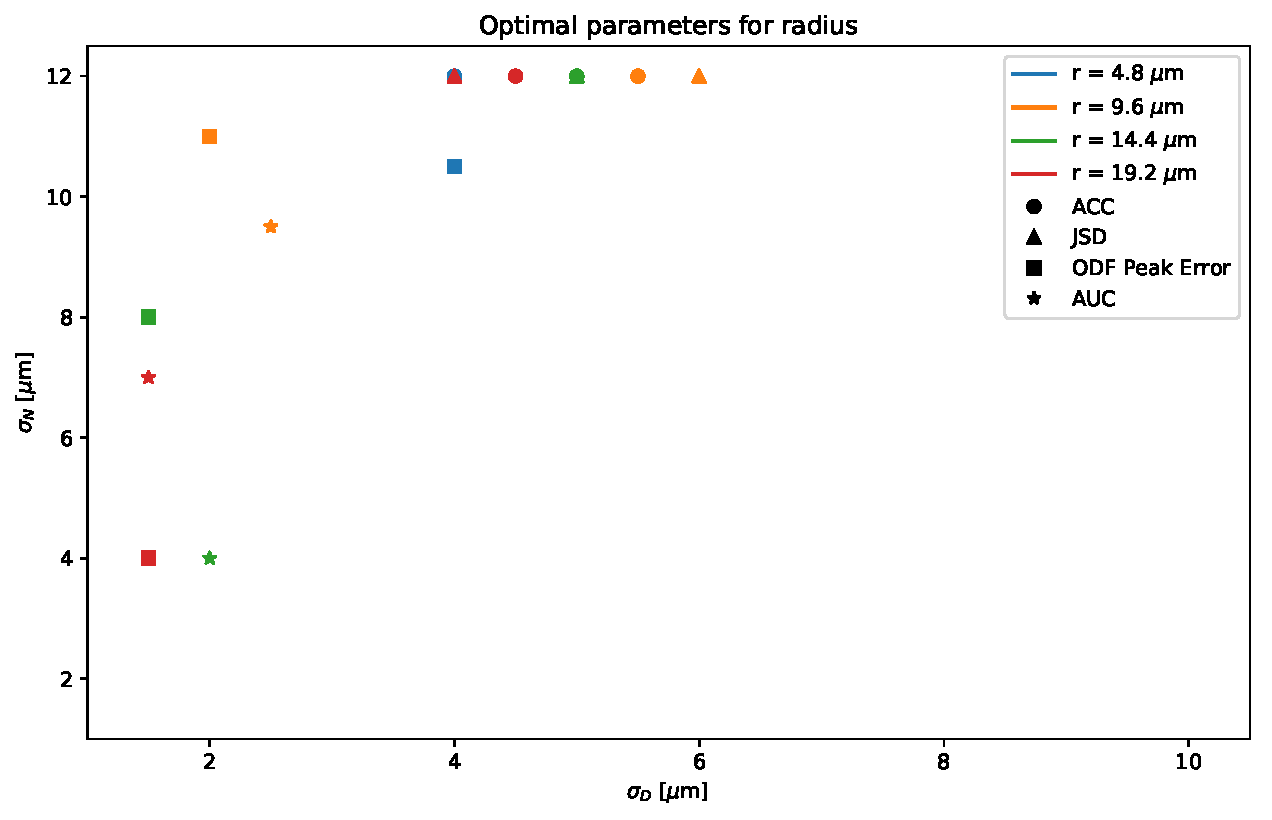
\includegraphics[width=0.7\linewidth]{../analysis/by_size_results/radius_best_params}
  \captionsetup{width=0.7\linewidth}
  \caption{Summary of Figure~\ref{fig:size_results}. Each point indicates the
    $\sigma_D$, $\sigma_N$ pair that maximizes a given metric for a given
    phantom. Different colors indicate different crossing angles and different
    shapes indicate different metrics.}
  \label{fig:size_max_inds}
\end{figure}

A few comments about these plots can be made. In general, all metrics are not
particularly sensitive to crossing angle or fiber size. The ACC and JSD appear
strongly correlated for all phantoms, and also show the most prominent ``peak''
in the parameter space. This peak is located around $\sigma_D$ = 7-8 $\upmu$m,
and around $\sigma_N$~=~6-9~$\upmu$m, with a slight increase in optimal $\sigma_N$
with higher crossing angles. The ACC and JSD show no trend and extremely
low parameter sensitivity for single-fiber phantoms of all sizes.

The AUC plots show nearly identical trends for all phantoms, but report
different optimal parameter selections than the ACC and JSD. There is a
less well-defined peak in the AUC plots, and it tends to be located at low 
$\sigma_D$ values (1-2 $\upmu$m) and low $\sigma_N$ values (3-4 $\upmu$m).
Ultimately, the AUC is based on the FA at each voxel, while the ODFs are
constructed from the orientations. For this reason, and since the AUC
reports different optimal parameters than the ODF-based metrics, the AUC
results can be effectively discarded. 

Note that both the JSD and Peak Error metrics depend on the discretization of
the sphere. This does not seem to have a large effect on the JSD, as it
correlates strongly with the ACC which is independent of spherical sampling.
The Peak Error, however, \textit{is} sensitive to the choice of spherical
sampling points, which I believe is why the Peak Error plots show discrete
regions. These regions do not show any sort of consistent trend across parameter
space or crossing angle. Note, however, that for each crossing angle phantom,
the Peak Error is generally within 5$^{\circ}$ for the parameters that maximize
the ACC and JSD. Note also that Peak Error does not appear sensitive at all to
the fiber radius; it is exactly 0$^{\circ}$ over nearly all of parameter space
for all single fiber population phantoms.

\section{Moving forward}
With the structure tensor parameters now in place, the following remains to be done:
\begin{itemize}
\item Choose FA threshold value
  \begin{itemize}
  \item Look at the same phantom data to choose the optimal FA threshold value. Voxels
    with FA below this threshold will be excluded from the ODF. 
  \end{itemize}
  \newpage
\item Verify HARDI reconstructions
  \begin{itemize}
  \item I have performed the following reconstructions using the ``default
    values'' in the Dipy python package: CSD, Q-ball (CSA), DTI and Sparse
    Fascicle.
  \item Talk with Sean and verify
  \end{itemize}
\item \textbf{Identify ROI to compare for poster}
  \begin{itemize}
  \item Will require \textit{some} form of registration.
  \item I suggest calculate the linear transform from 5 $\upmu$m x-ray data to 50 $\upmu$m structural MRI
  \item Apply this data to the 1.2 $\upmu$m x-ray data
  \item Compare ODFs (potentially just qualitatively) 
  \end{itemize}
\end{itemize}


\section{Conclusion}
This study has demonstrated the feasibility of performing quantitative 3D
validation of dMRI FODs with synchrotron x-ray data. This marks the first
available ground truth dataset and methodology to allow for whole-brain
validation of dMRI FODs with natively isotropic resolution and no sectioning. The
application of this analysis to a whole mouse brain will provide a wealth of
information regarding the ability of different dMRI algorithms to represent
microstructural regions of varying complexity, and will provide the means to
perform future large-scale validation studies in dMRI, tractography, and
connectomics.


\bibliographystyle{ieeetr}
\bibliography{reportbib}
\end{document}
